\documentclass{article}
\usepackage{mathtools}
\usepackage{pgfplots}
\usepackage{natbib}
\usepackage{graphicx}

\usepackage[utf8]{inputenc}

\title{CSE546 HW0 A}
\author{Bobby Deng | 1663039 | dengy7 }
\date{March 2020}


\begin{document}

\maketitle

\section{A.1}

\[ P(A|B)=\frac{P(A)*P(B|A)}{P(B)} \]
\[ P(B)=P(A)*P(B|A)+P(A^-)*P(B|A^-) \]
\[ P(A^-)=1-P(A)\]

$A$: You have the disease. $A^-$: You don't have the disease.

$B$: Test is positive. $B^-$: Test is negative.

$P(A)=0.0.0001$, $P(A^-)=0.9999$

\[ P(B)= P(A)*P(B|A)+P(A^-)*P(B|A^-) \]
\[ P(B)= 0.0001*0.99+0.9999*0.01 \]
\[ P(B)= 0.010098 \]

\[ P(A|B)=\frac{P(A)*P(B|A)}{P(B)} \]
\[ P(A|B)=\frac{0.0001*0.99}{0.010098} \]
\[ P(A|B)=0.0098 \]


\section{A.2}
\subsection{a.}
\[ Cov(X,Y)=E[(X-E[X])(Y-E(Y))] \]
\[ Cov(X,Y)=E[XY-XE[Y]-YE[X]+E[X]E[Y]] \]
\[ Cov(X,Y)=E[XY]-E[X]E[X+Y]+E[X]E[Y] \]
\[ Cov(X,Y)=E[XY]-E[X](E[X]+E[Y])+E[X]E[Y] \]
\newline

1. \textbf{When $E[Y|X=x]=x$, then $E[X]=E[Y]$, so we can change all $E[Y]$ to $E[X]$.}
\[ Cov(X,Y)=E[XY]-E[X](E[X]+E[X])+E[X]E[Y] \]
\[ Cov(X,Y)=E[XX]-E[X]E[X+X]+E[X]^2 \]
\[ Cov(X,Y)=E[XX-XE[X]-XE[X]+E[X]^2] \]
\[ Cov(X,Y)=E[(X-E[X])(X-E(X))] \]
\[ Cov(X,Y)=E[(X-E[X])^2] \]

\subsection{b.}
When X,Y are independent:
\[ Cov(X,Y)=E[XY-XE[Y]-YE[X]+E[X]E[Y]] \]
\[ Cov(X,Y)=E[XY]-E[X]E[Y]-E[Y]E[X]+E[X]E[Y] \]\newline

1. We know that $E[XY]=E[X]E[Y]$, Then 
\[ Cov(X,Y)=0 \]

\section{A.3}
\subsection{a.}
Since $Z=X+Y$, the probability function for Z should be joint probability of X and Y.

\[ h(z) = P(Z);Z=X+Y \]
\[ Y=0,X=Z;Y=1,X=Z-1;Y=2,X=Z-2;....;Y=Z-1,X=1;Y=0,X=Z \]
Since X,Y are independent, then
\[h(z)=\sum_0^Z P(X=i,Y_k=Z-i)\]
\[h(z)=\sum_0^Z P(X=i)*P(Y=Z-i)\]
\[h(z)=\sum_0^Z f(x)*g(y)\]
Above is showing what happened for discrete variable. It is the same story for continuous variable, however there are infinite many of that variable X,Y combination. So, we need to use integral to represents the infinite many variables and the area under it which representing the probability of a single Z.  

\[ h(z)=\int_{-\infty}^{\infty} f(x)*g(y) \]

We know that $Z=X+Y$, so we can replace $Y=Z-X$, then it becomes:
\[ h(z)=\int_{-\infty}^{\infty} f(x)*g(z-x) \]

\subsection{b.}
First of all, Z can not be less than 0 or bigger than 2 since X,Y are on [0,1].

Then we look at Z in [1,2] and Z in [0,1] separately.

$f(x)*g(z-x)$ Could either equal to 0 or 1.

When X and Z-x are both on the designated interval, $f(x)*g(z-x)=1$, 0 otherwise.

Now we only look at situations where it is 1. 

When $1\ge x \ge0$ or $1\ge Z-X \ge 0$

Then we get two intervals: $Z\ge X \ge 0$ and $1\ge X \ge Z-1$\newline

We Get:
\[ h(z)=\int_{0}^{Z} 1dx = z\]
\[ h(z)=\int_{Z-1}^{1} 1dx = 2-z\]


\[ 
h(z) = \begin{cases}
z & \text{for $0 < z < 1$} \\
2-z & \text{for $1 \le z < 2$} \\
0 & \text{otherwise.}
\end{cases} 
\]

\section{A.4}
We want $E[Y]=0$ and $var(Y)=\sigma^2=1$
\[ E[Y]=aE[X]+b=0\]
\[ 0=a\mu+b\]
\[ b=-a\mu\]
\[ var(Y) = var(aX+b) =1\]
\[ var(y) = a^2var(X) + var(b)=1\]
\[ var(y) = a^2\sigma^2 + 0=1\]
\[ var(y) = a^2\sigma^2=1\]
\[ a^2 = 1/\sigma^2\]
\[a=1/\pm \sigma\]
So, 
\[b=\mu / \pm \sigma\]

\section{A.5}
\[ E[\hat{\mu}_n] = E[\frac{1}{n}\sum_{i=1}^nX_i] = \frac{1}{n}\sum_{i=1}^nE[X_i] = \frac{1}{n}\sum_{i=1}^n\mu = \mu \]

\[ var(\hat{\mu}_n) = var(\frac{1}{n}\sum_{i=1}^n X_i)=\frac{1}{n^2}var(\sum_{i=1}^nX_i)=\frac{1}{n^2}\sum_{i=1}^nvar(X_i)=\frac{1}{n^2}\sum_{i=1}^n\sigma^2=\frac{\sigma^2}{n}\]
Now we know $E[\hat{\mu}_n]=\mu$ and $var(\hat{\mu}_n)=\frac{\sigma^2}{n}$. We can use the above calculation for the equations below.
\[ E[Z] = E[\sqrt{n}(\hat{\mu}_n-\mu)] = E[\sqrt{n}](E[\hat{\mu}_n] - E[\mu]) = \sqrt{n}(\mu - \mu) = 0\]

\[ var(Z)=var(\sqrt{n}(\hat{\mu}_n-\mu)) = n*var(\hat{\mu}_n-\mu)\] \[=n*E[((\hat{\mu}_n-\mu)-E[\hat{\mu}_n-\mu])^2] \]
\[=n*E[((\hat{\mu}_n-\mu)-0)^2] \]
\[=n*E[(\hat{\mu}_n-\mu)^2] \]
\[=n*var(\hat{\mu}_n)\]
\[=\sigma^2\]


\section{A.6}
\subsection{a.}
\[\hat{F_n}(x)= \frac{1}{n}\sum_{i=1}^n1\{X_i\le x\}\]
\[E[\hat{F_n}(x)]= E[\frac{1}{n}\sum_{i=1}^n1\{X_i\le x\}] = \frac{1}{n}\sum_{i=1}^nE[1\{X_i\le x\}] \]

Lets work out what $E[1\{X_i\le x\}]$ is:
\[ E[1\{X_i\le x\}] = \int_{-\infty}^{\infty} 1\{X_i\le x\}*f(x) dx \]

\[ = \int_{-\infty}^{\infty}1*f(x) dx; \;\;\;when X_i\le x\]

\[ = F(x); \;\;\;when X_i\le x \]

Now:
\[ E[\hat{F_n}(x)]= \frac{1}{n}\sum_{i=1}^nE[1\{X_i\le x\}] = \frac{1}{n}\sum_{i=1}^nF(x)=F(x)\]

\subsection{b.}
\[ var(\hat{F_n}(x))=E[(\hat{F_n}(x) -F(x))^2] = E[(\hat{F_n}(x) -F(x))(\hat{F_n}(x) -F(x))] \]
\[ =E[\hat{F_n}(x)^2-2\hat{F_n}(x)F(x)+F(x)^2] \]

\[ var(\hat{F_n}(x))= var(\frac{1}{n}\sum_{i=1}^n1\{X_i\le x\}) = \frac{1}{n^2}\sum_{i=1}^nvar(1\{X_i\le x\}) \]
Lets work out what $var(1\{X_i\le x\})$ (Let A to represent it)is: 
\[ var(A) = E[(A-E[A])^2]\]
\[ var(A) = E[A^2 -2AE[A]+(E[A])^2]\]
Since $A$ is 1, so $A^2=A$ :
\[ var(A) = E[A] -2E[A]E[A]+(E[A])^2] \]
\[ var(A) = E[A] -E[A]E[A]] \]
\[ var(A) = F(x) - F(x)^2 \]
\[ var(A) = F(x)(1-F(x)) \]

\[var(\hat{F_n}(x))=\frac{1}{n^2}\sum_{i=1}^nvar(1\{X_i\le x\})=\frac{1}{n^2}\sum_{i=1}^nF(x)(1-F(x))\]
\[ var(\hat{F_n}(x))=\frac{F(x)(1-F(x))}{n}\]

\subsection{c.}

\[ var(\hat{F_n}(x))=E[(\hat{F_n}(x)-F(x))^2] =\frac{F(x)(1-F(x))}{n}\]
Prove if $\frac{F(x)(1-F(x))}{n}\le\frac{1}{4n}$.
Which is same as prove: $F(x)(1-F(x))<\frac{1}{4}$.\newline

\[ F(x)(1-F(x)) = \frac{1}{4}-\frac{1}{4}+F(x)^2-F(x) \]

\[ F(x)(1-F(x)) = \frac{1}{4}-(\frac{1}{2}-F(x))^2 \le \frac{1}{4}\]
Which is same as:
\[\frac{F(x)(1-F(x))}{n}\le\frac{1}{4n}\]



\section{A.7}
\subsection{a.}
Rank for A is: 2.\newline
Rank for B is: 2.
\subsection{b.}
$A^T=\begin{bmatrix}
1 & 1 & 1\\
2 & 0 & 1\\
1 & 3 & 2
\end{bmatrix}$
=
$\begin{bmatrix}
1 & 1 & 1\\
2 & 0 & 1\\
0 & 2 & 1
\end{bmatrix}$
=
$\begin{bmatrix}
1 & 0 & 1/2\\
0 & 1 & 1/2\\
0 & 0 & 0
\end{bmatrix}$ \newline


So the minimal basis for A: 
$\begin{bmatrix}
1\\ 
0\\
1/2
\end{bmatrix}$
and
$\begin{bmatrix}
0\\ 
1\\
1/2
\end{bmatrix}$ \newline


$B^T=\begin{bmatrix}
1 & 1 & 1\\
2 & 0 & 1\\
1 & 3 & 2
\end{bmatrix}$
=
$\begin{bmatrix}
1 & 1 & 1\\
0 & 2 & 1\\
0 & 0 & 0
\end{bmatrix}$
=
$\begin{bmatrix}
1 & 0 & 1/2\\
0 & 1 & 1/2\\
0 & 0 & 0
\end{bmatrix}$\newline


So the minimal basis for B: 
$\begin{bmatrix}
1\\ 
0\\
1/2
\end{bmatrix}$
and
$\begin{bmatrix}
0\\ 
1\\
1/2
\end{bmatrix}$


\section{A.8}
\subsection{a.}

$\begin{bmatrix}
0 & 2 & 4\\
2 & 4 & 2\\
3 & 3 & 1
\end{bmatrix}$
$\begin{bmatrix}
1 & 1 & 1
\end{bmatrix}^T$
=
$\begin{bmatrix}
0 & 2 & 4\\
2 & 4 & 2\\
3 & 3 & 1
\end{bmatrix}$
$\begin{bmatrix}
1\\
1\\
1
\end{bmatrix}$
=
$\begin{bmatrix}
6\\
8\\
7
\end{bmatrix}$

\subsection{b.}
$\left[\begin{array}{ccc|c}
0 & 2 & 4 & -1\\
2 & 4 & 2 & -2\\
3 & 3 & 1 & -4
\end{array}\right]$\newline
Solution to this augmented matrix is:
$\begin{bmatrix}
-2\\
1\\
-1
\end{bmatrix}$

\section{A.9}
\subsection{a.}
Based on the relationship, we can get this:
$\begin{bmatrix}
-1 & 2
\end{bmatrix}$
*
$\begin{bmatrix}
x_1\\
x_2
\end{bmatrix}$
+2=0 \newline

Then we can get the relationship $x_1 = 2x_2+2$.

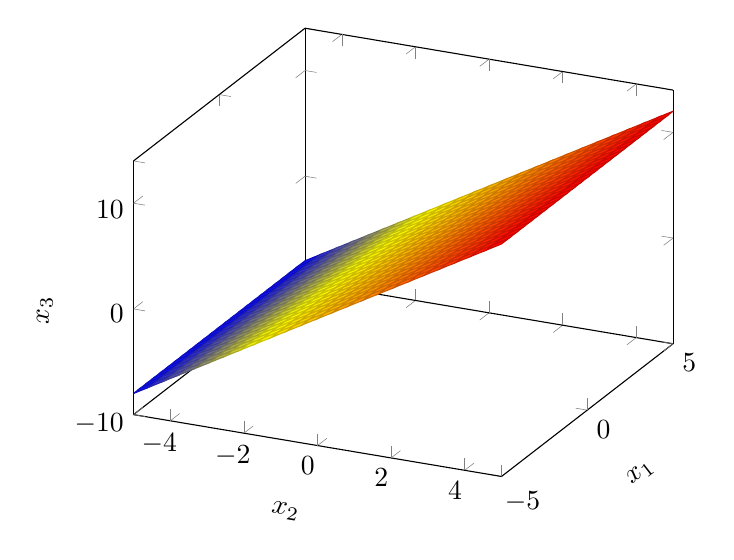
\begin{tikzpicture}
	\begin{axis}[
		xlabel=$x_2$,
		ylabel=$x_1$,
		zlabel=$x_3$,
		xlabel style={sloped like x axis},
		ylabel style={sloped}
	]
	\addplot3[surf] {2*x+2};
	\end{axis}
\end{tikzpicture}


\subsection{b.}
$\begin{bmatrix}
1 & 1 & 1
\end{bmatrix}$
*
$\begin{bmatrix}
x_1\\
x_2\\
x_3
\end{bmatrix}$
+0=0 \newline

Then we can get the relationship $x_1 = -x_2-x_3$.

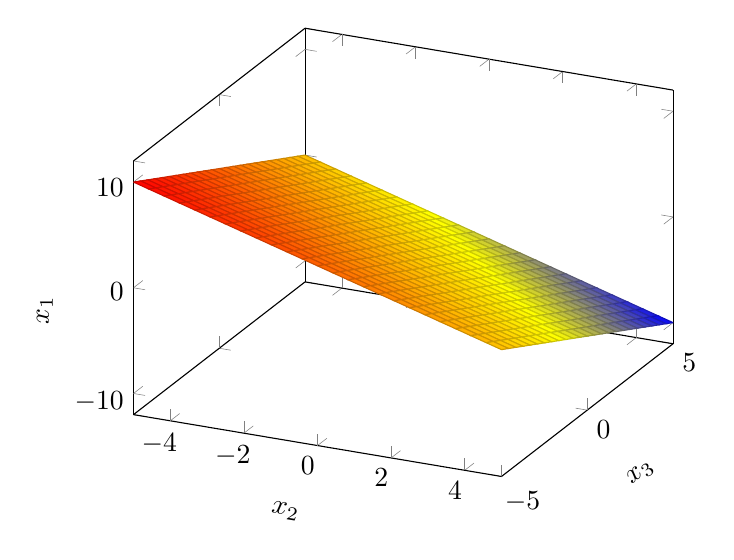
\begin{tikzpicture}
	\begin{axis}[
		xlabel=$x_2$,
		ylabel=$x_3$,
		zlabel=$x_1$,
		xlabel style={sloped like x axis},
		ylabel style={sloped}
	]
	\addplot3[surf] {-x-y};
	\end{axis}
\end{tikzpicture}

\subsection{c.}

When $\Tilde{x}_0$ is the minimizer, $x=\Tilde{x}_0$ 
\[\min_{x}\begin{Vmatrix}
$x_0-x$
\end{Vmatrix}^2
=
\begin{Vmatrix}
$x_0-\Tilde{x}_0$
\end{Vmatrix}^2
=
\begin{vmatrix}
\frac{(w^T x_0-w^T\Tilde{x}_0)}{w^T w}  
\end{vmatrix}^2 
=
(
\frac{w^T x_0-w^T\Tilde{x}_0}{w^T w}  
)^2 
\]
Since $w^T x + b=0$, then $w^T \Tilde{x}_0 + b=0$,   \newline
Then $b=-w^T \Tilde{x}_0$.  \newline
\[(
\frac{w^T x_0-w^T\Tilde{x}_0}{w^T w}  
)^2 
=
(\frac{w^T x_0+b}{w^T w}  
)^2 
\]
So the square distance is $(\frac{w^T x_0+b}{w^T w}  
)^2 $.


\section{A.10}
\subsection{a.}
\[x^T Ax
=
\begin{bmatrix}
x_1 & \dots & x_n
\end{bmatrix}
\begin{bmatrix}
A_{1,1} & \dots & A_{1,n}\\
\vdots & \ddots & \vdots\\
A_{n,1} & \dots & A_{n,n}
\end{bmatrix}
\begin{bmatrix}
x_1\\
\vdots\\
x_n
\end{bmatrix}\]

\[  
=
\begin{bmatrix}
\sum_{i=1}^n x_i A_{i,1} & \dots & \sum_{i=1}^n x_i A_{i,n}
\end{bmatrix}
\begin{bmatrix}
x_1\\
\vdots\\
x_n
\end{bmatrix}
=
\sum_{j=1}^n (x_j (\sum_{i=1}^n x_i A_{i,j}))
\]

For $y^T Bx$, it is the similar story, \newline
\[ \
y^T Bx
=
\sum_{j=1}^n (x_j (\sum_{i=1}^n y_i B_{i,j})) \]
So, 

\[ f(x,y)= x^T Ax + y^T Bx + c
=
\sum_{j=1}^n (x_j (\sum_{i=1}^n x_i A_{i,j}))+\sum_{j=1}^n (x_j (\sum_{i=1}^n y_i B_{i,j}))+c
=
\]

\[
=
\sum_{j=1}^n (x_j (\sum_{i=1}^n x_i A_{i,j})+(\sum_{i=1}^n y_i B_{i,j}))+c
=
\sum_{j=1}^n (x_j \sum_{i=1}^n (x_i A_{i,j}+ y_i B_{i,j}))+c
\]

\subsection{b.}
\[
\nabla_z f(x,y)=
\begin{bmatrix}
\frac{\partial f(x,y)}{\partial z_1} &
\dots &
\frac{\partial f(x,y)}{\partial z_n}
\end{bmatrix}^T
\]

\[
\nabla_x f(x,y)=
\begin{bmatrix}
\frac{\partial f(x,y)}{\partial x_1} &
\dots &
\frac{\partial f(x,y)}{\partial x_n}
\end{bmatrix}^T
\]

Let's look at each $\frac{\partial f(x,y)}{\partial x_k}$ separately, and use k here in order to differentiate the i from matrix.\newline

Since $f(x,y)=\sum_{j=1}^n (x_j \sum_{i=1}^n (x_i A_{i,j}+ y_i B_{i,j}))+c$:


\begin{equation}
\begin{split}
\frac{\partial}{\partial x_k} & = \frac{\partial f(x,y)}{\partial x_k}(\sum_{j=1}^n (x_j \sum_{i=1}^n (x_i A_{i,j}+ y_i B_{i,j}))+c) \\
 & = \sum_{j=1}^n \frac{\partial}{\partial x_k}[(x_j \sum_{i=1}^n (x_i A_{i,j}+ y_i B_{i,j}))+c] \\
 & = \sum_{j=1}^n \frac{\partial}{\partial x_k}(x_j \sum_{i=1}^n (x_i A_{i,j}+ y_i B_{i,j})) + 0 \\
 & = \sum_{j=1}^n \frac{\partial}{\partial x_k}(x_j \sum_{i=1}^n (x_i A_{i,j}+ y_i B_{i,j})) \\
 & = \sum_{j=1}^n [\frac{\partial}{\partial x_k}(x_j)( \sum_{i=1}^n (x_i A_{i,j}+ y_i B_{i,j}))+\frac{\partial}{\partial x_k}(\sum_{i=1}^n (x_i A_{i,j}+ y_i B_{i,j}))(x_j)] \\
 & = \sum_{j=1}^n \frac{\partial}{\partial x_k}(x_j)( \sum_{i=1}^n (x_i A_{i,j}+ y_i B_{i,j}))+ \sum_{j=1}^n \frac{\partial}{\partial x_k}(\sum_{i=1}^n (x_i A_{i,j}+ y_i B_{i,j}))(x_j) \\
 & = [0+0+\frac{\partial}{\partial x_k}(x_k)( \sum_{i=1}^n (x_i A_{i,k}+ y_i B_{i,k}))+\dots+0+0]+[\sum_{j=1}^n(x_j \sum_{i=1}^n \frac{\partial}{\partial x_k}(x_i A_{i,j})+0)] \\
 & = \sum_{i=1}^n (x_i A_{i,k}+ y_i B_{i,k}) + \sum_{j=1}^n x_j (0+0+\frac{\partial}{\partial x_k}(x_k A_{k,j})+0+\dots+0+0) \\
 & = \sum_{i=1}^n (x_i A_{i,k}+ y_i B_{i,k}) + \sum_{j=1}^n x_j (\frac{\partial}{\partial x_k}(x_k A_{k,j})) \\
 & = \sum_{i=1}^n (x_i A_{i,k}+ y_i B_{i,k}) + \sum_{j=1}^n x_k A_{k,j} - They are all from 1-n \\
 & = \sum_{i=1}^n (x_i A_{i,k}+ y_i B_{i,k} + x_k A_{k,i})
\end{split}
\end{equation}

So,

\begin{equation}
\begin{split}
\nabla_x f(x,y) & = \begin{bmatrix}
\frac{\partial f(x,y)}{\partial x_1} &
\dots &
\frac{\partial f(x,y)}{\partial x_n}
\end{bmatrix}^T \\
& = \begin{bmatrix}
\sum_{i=1}^n (x_i A_{i,1}+ y_i B_{i,1} + x_1 A_{1,i}) &
\dots &
\sum_{i=1}^n (x_i A_{i,n}+ y_i B_{i,n} + x_k A_{n,i})
\end{bmatrix}^T
\end{split}
\end{equation}


\subsection{c.}
\[
\nabla_y f(x,y)=
\begin{bmatrix}
\frac{\partial f(x,y)}{\partial y_1} &
\dots &
\frac{\partial f(x,y)}{\partial y_n}
\end{bmatrix}^T
\]

Now, do the same thing as x. \newline

\begin{equation}
\begin{split}
\frac{\partial f(x,y)}{\partial y_k} & = \frac{\partial}{\partial y_k}(\sum_{j=1}^n (x_j \sum_{i=1}^n (x_i A_{i,j}+ y_i B_{i,j}))+c) \\
& = \sum_{j=1}^n x_j(\frac{\partial}{\partial y_k}(\sum_{i=1}^n (x_i A_{i,j}+ y_i B_{i,j}))) \\
& = \sum_{j=1}^n x_j (0+0+[0+\frac{\partial}{\partial y_k}(y_k B_{k,j})]+0+\dots + 0)\\
& = \sum_{j=1}^n x_j B_{k,j}
\end{split}
\end{equation}

So we can get, 
\begin{equation}
\begin{split}
\nabla_y f(x,y) & = \begin{bmatrix}
\frac{\partial f(x,y)}{\partial y_1} &
\dots &
\frac{\partial f(x,y)}{\partial y_n}
\end{bmatrix}^T \\
& = \begin{bmatrix}
\sum_{j=1}^n x_j B_{1,j} &
\dots &
\sum_{j=1}^n x_j B_{n,j}
\end{bmatrix}^T
\end{split}
\end{equation}




\section{A.11}
\subsection{a.}
\includegraphics[scale=0.7]{11a.png}

\subsection{b.}
\includegraphics[scale=0.7]{11b.png}

\section{A.12}
\subsection{a.}
According to previous answer: $var(\hat{F_n}(x))\le\frac{1}{4n}$, so:

\begin{equation}
\begin{split}
\sqrt{var(\hat{F_n}(x))}\le 0.0025 \\
var(\hat{F_n}(x)) \le & (0.0025)^2 \\
var(\hat{F_n}(x)) \le & \frac{1}{4n} \\
(0.0025)^2 = & \frac{1}{4n} \\ 
n = & 4000
\end{split}
\end{equation}

\includegraphics[scale=0.5]{12a.png}

\subsection{b.}
\includegraphics[scale=0.5]{12b.png}


\end{document}
